\documentclass[12pt]{article}
\usepackage{amsmath, amssymb, amsfonts, amsthm}
\usepackage{graphicx, tabularx, geometry, minted}
\usepackage{caption, float}
\usepackage{setspace, lipsum}
\usepackage[table]{xcolor}

\usepackage{tikz, pgfplots}
\pgfplotsset{compat=1.18}

\geometry{top=1 in, bottom=1 in, left=1 in, right=1 in}

% \onehalfspacing

\theoremstyle{definition}
\newtheorem{theorem}{Theorem}
\newtheorem{definition}{Definition}
\newtheorem{lemma}{Lemma}
\newtheorem{proposition}{Proposition}
\newtheorem{remark}{Remark}
\newtheorem{corollary}{Corollary}
\newtheorem{problem}{Problem}
\newtheorem{example}{Example}

% \setlength\parindent{0 pt}

\begin{document}

\begin{titlepage}
    \begin{center}
        \vspace*{2 cm}

        \begin{spacing}{2}
            {\Large \textbf{Polynomial Root-Finding Methods: \\ Theory, Weaknesses, and Wilkinson's Polynomial}}
        \end{spacing}

        \vspace*{1 cm}

        {\large Joel Penney} \par

        \vspace*{0.25 cm}
        
        \texttt{jscottp@mun.ca}

        \vfill

        \begin{abstract}
            This paper studies six algorithms used to solve root-finding problems involving single-variable polynomials. Specifically, we consider theoretical foundations such as the intermediate value theorem as well as the details of iterative rules to explain the differences between several bracketed and open methods. The six algorithms are also compared under challenging circumstances such as flat regions and Wilkinson's polynomial. We find that no algorithm performs consistently better than all of the others, although TOMS748 and Halley's method are often able to locate roots quickly. As we demonstrate, the structure of the root-finding problem influences the chosen approach, relevant theory considered, and the methods applied to efficiently find roots.
        \end{abstract}

        \vfill

        \begin{spacing}{1.5}
            Memorial University of Newfoundland \par
            Department of Mathematics and Statistics \par
            MATH 3030: Mathematical Inquiry II
        \end{spacing}

        \vspace*{1.25 cm}

        January 29, 2026

        \vspace*{0.25 cm}
    \end{center}
\end{titlepage}

% \tableofcontents
% \newpage

\section{Introduction}
\noindent
Suppose you are a physicist, studying the trajectory of a projectile as it flies through the air. Alternatively, picture yourself as a biological researcher trying to model the spread of disease in a population. Perhaps, in another case, you want to analyze costs and predict economic patterns to ensure your financial decisions are well-informed. In all of these cases, polynomials have been used to represent a real situation or phenomenon. 

The roots of polynomials, or inputs that result in an output of zero, frequently have important physical or scientific meaning. Often, determining them is a problem for numerical analysis, an area of mathematics concerned with solving problems in numerical form using a constructive computational procedure \cite{gautschi2011numerical}. Various methods, known as root-finders, are commonly used today and include matrix methods, functional iterations, and hybrid methods \cite{pan2007real}. We start by considering the underlying theory for determining polynomial roots. After closely examining the bisection method and Newton's method, we combine computational approaches with crucial theory to solve root-finding problems. In doing so, we are able to see strengths and weaknesses of various root finders. Finally, we challenge six root-finding methods to determine the zeros of Wilkinson's polynomial, a notoriously difficult polynomial in root-finding. 

To find polynomial roots numerically is to engage in a long line of work that is still of great interest today. The mathematics behind polynomial root-finding is very valuable, and has played an important role in many modern disciples such has computer technology and engineering \cite{naseem2022novel}.

\section{Methods}

\subsection{Preliminaries}
\noindent
Suppose we know a function $f$ and want to determine the value or values of $x$ such that \[f(x)=0.\]

We may first try analytical methods to determine $x$, which is often convenient if $f$ is sufficiently basic, such as a polynomial of degree 1 or 2. Frequently, however, our function $f$ is more complicated or sophisticated, and analytical methods are impractical or unavailable. Instead, numerical methods are often imposed on \textit{root-finding problems} such as the one described. Root-finding algorithms (or root-finding methods) are used to approximate the roots or zeros of a function, with the requirement that the function be continuous. Additionally, solving the equation \[g(x)=h(x)\] is equivalent to finding the roots of $f(x)=g(x)-h(x)$, which shows how widespread root-finding problems are and how important root-finding methods can be. 

\begin{definition}
    A \textit{polynomial of one variable}, denoted $p(x)$, is an expression that can be written in the form \[a_nx^x + a_{n-1}x^{x-1} + \cdots +a_1x + a_0\] where $a_n, ..., a_0$ are coefficients, $a_n$ is nonzero, $x$ is a variable, and $n$ is the degree \cite{kalantari2008polynomial}. If the coefficients are real and the variable is restricted to the real numbers, then the expression is called a \textit{real polynomial}. The equation $p(x)=0$ is called a \textit{polynomial equation}.
\end{definition}

Each polynomial of one variable (or just polynomial for short) is continuous everywhere.

\begin{theorem}[Fundamental Theorem of Algebra]
    Every nonzero polynomial of one variable with complex coefficients has exactly $n$ complex roots when multiplicity is counted.
\end{theorem}

Many proofs of this famous theorem exist. They can be found in  \cite{steed2015proofs}, for example. Although we are primarily interested in \textit{real} roots, the theorem indicates exactly how many (complex) roots a polynomial must have, which is helpful for determining the set of all roots.

\subsection{The Bisection Method}
\noindent
The bisection method is one of the earliest methods used to find the roots of the equation $f(x)=0$ \cite{solanki2014role}. This method can only be applied to a function $f$ if it continuous on an interval $[a,b]$, and $f(a)$ and $f(b)$ have opposite signs. In this case, $a$ and $b$ are said to form a \textit{bracket} for the function. On $[a,b]$, then, the function $f$ has at least one root by the intermediate value theorem. More precisely, a corollary of this theorem known as \textit{Bolzano's theorem} states that a continuous $f$ on $[a,b]$ with $f(a)$ and $f(b)$ of opposite signs must have at least one $c \in (a,b)$ such that $f(c)=0$. For this reason, the bisection method is guaranteed to find a root, provided the continuity and sign requirements are met and the process is not limited by a maximum number of iterations or steps.

Now we explain the bisection algorithm. First, we check that the function values at the endpoints have opposite signs. If they have the same sign (that is, $f(a)\cdot f(b) >0$), then the method cannot be applied. Note that if $f(a)$ or $f(b)$ are zero, then a root is found. Otherwise, we calculate the midpoint $m$ of the interval by \[m=\frac{a+b}{2}\] and check if it is a root. If it is not, then we check if $f(m)$ has the same sign as $f(a)$, in which case $a$ is replaced by $m$. Else, $b$ is replaced by $m$. A new midpoint is then calculated and the process repeats.

This algorithm is written in Python in Appendix \ref{manualalgorithms}. To our function called \texttt{bisection} we give the bracket as well as two other variables: tolerance and the maximum number of iterations. If the value of the function is extremely close to zero, then the algorithm should terminate since a root is found. Alternatively, if the width of the bracket becomes extremely small, the process should stop as well, as this is a usual test that indicates a root has been located \cite{naseem2022novel}. Thus, the lines
\begin{verbatim}
    if abs(f(mid)) < tolerance or abs(b-a) < tolerance:
      return mid, points
\end{verbatim}
show how the function stops and returns the approximate root \texttt{mid} (as well as a list of previous approximations called \texttt{points}).

There are other methods that use a bracket and the intermediate value theorem to ensure a root will be found if it is known to be in an interval. Brent's method is a hybrid method that switches between the bisection method and two other methods to (ideally) locate the root faster. TOMS748, an algorithm published in ACM Transactions on Mathematical Software (TOMS), is another modern method that uses multiple other algorithms for faster convergence, typically \cite{alefeld1995algorithm}.

\subsection{Newton's Method}
\noindent
Another popular root-finding method was developed by Newton and first printed in 1685, before Joseph Raphson reformulated the technique in 1690 \cite{sutherland1989finding}. Newton's method (or the Newton-Raphson method) starts with an initial guess $x_0$ and forms a better approximation $x_1$ of the root for a real-valued function $f$ by drawing the tangent line of the function at $(x_0, f(x_0))$ and letting $x_1$ be the point where the tangent line meets the $x$-axis \cite{sutherland1989finding}. We repeat this process iteratively, using the rule \[x_{i+1} = x_i - \frac{f(x_i)}{f'(x_i)}.\]

This key rule is easily written in Python as
\begin{verbatim}
    xnew = x0 - (f(x0)/df(x0))
\end{verbatim}
and we loop over the maximum number of iterations until a root is found within the given tolerance. While this method is known to usually converge quick, there are three main difficulties we can identify at this stage. First, and unlike the bisection method, convergence upon a root or a desired root is not guaranteed. This is an \textit{open method}, and we see some of its associated struggles in the Results section. Second, the rule requires that the function has a derivative $f'$. Third, the derivative must not be zero at the initial guess or subsequent approximations, or else division by zero would occur. Our algorithm acknowledges this final difficulty and will not return a root if a derivative of zero occurs:
\begin{verbatim}
    if abs(df(x0)) < 1e-10:
      print("Error: Derivative is zero.")
      return None, points
\end{verbatim}

Secant method is another open method that uses a secant line instead of a tangent line. Its rule \[x_{i+1} = x_i - f(x_i)\frac{x_i - x_{i-1}}{f(x_i) - f(x_{i-1})}\] requires two points instead of a derivative. Our program for comparing all of the methods uses the \texttt{SciPy} package. Each of the root-finders returns the approximate root (if found) followed by a \texttt{RootResults} object from which we can extract important data and use to plot graphs. Omitting the derivative in the Newton's method function causes it to run secant method instead:
\begin{verbatim}
    root, secantinfo = scipy.newton(f, x0, maxiter=500, full_output=True)
\end{verbatim}
Likewise, Halley's method is a variation that uses the rule \[x_{i+1} = x_i - \frac{2f(x_i)f'(x_i)}{2[f'(x_i)]^2 - f(x_n)f''(x_n)}\] and must be supplied a first and second derivative:
\begin{verbatim}
    root, halleyinfo = scipy.newton(f, x0, fprime=df, fprime2=ddf, 
                                    maxiter=500, full_output=True)
\end{verbatim}

The bisection method and Newton's method have been programmed manually in order to more precisely examine how they work. In a second Python notebook, all six of the methods mentioned have been implemented using \texttt{SciPy}. This sets a great framework for studying their strengths, efficiency, and how they sometimes fail.

\section{Results}

\subsection{Visualizing Root-Finding Algorithms}
\noindent
First, we want to visualize our two main methods in action. We do this by plotting the root approximations after every iteration. Consider the polynomial $p_1(x) = x^3-7x$. In this opening example, the three roots, $0, \sqrt{7}$, and $-\sqrt{7}$, are easily found algebraically.

\begin{figure}[h]
    \centering
    \includegraphics[width=0.75\linewidth]{images/greatstart.png}
    \caption{Typical root-finder behaviour on the polynomial $p_1(x) = x^3-7x$ with $x_0=-4.5$ for Newton's method and bracket $[2, 4]$ for the bisection method.}
    \label{greatstart}
\end{figure}

With our tolerance set to $10^{-12}$, both root-finders perform well and Newton's method takes only 7 iterations. It is usual for Newton's method to converge quickly (i.e., requiring less iterations) when the initial guess is close. Bisection converges less quickly in this example, with guesses on either side of the (true) root before the algorithm reaches the stopping criteria. Note that in this example the bisection method and Newton's method produce accurate, usable decimal approximations of $\sqrt{7}$ and $-\sqrt{7}$, respectively.

Suppose we want to determine the set of all real roots of the polynomial \[p_2(x) = x^6 - 2x^5 - 3x^4 + 4x^3 + 5x^2 + x - 7\] with real coefficients. Numerical methods are highly useful here. By the Fundamental Theorem of Algebra, there are 6 complex roots, some of which may be real. With the polynomial written in descending order as above, we count 3 changes in the signs of the leading coefficients. Thus, by Descartes' Rule of Signs, there are 3 or 1 positive real roots (as well as 3 or 1 negative real roots). Testing some small positive values of $x$ we find that
\begin{align*}
    p_2(1) &= -1 <0,\\
    p_2(1.5) &= 0.265625 >0,\\
    p_2(2) &= -1 <0,\\
    p_2(2.5) &= 20.890625 >0.
\end{align*}

By Bolzano's theorem, then, there are roots on the intervals $(1, 1.5), (1.5, 2)$, and $(2, 2.5)$. The bisection method can easily find (any of) these, as shown in Figure \ref{newpolynomial}.

\begin{figure}[h]
    \centering
    \includegraphics[width=0.75\linewidth]{images/newpolynomial.png}
    \caption{The degree six polynomial $p_2(x)$ with bracket $[1, 1.5]$ and $x_0=-1.75$.}
    \label{newpolynomial}
\end{figure}

If we examine negative $x$-values, we find that there is only one sign change and that it is somewhere around $-1.5$ (Newton's method is then well-suited to approximate this root). We conclude that there are 3 positive real roots, 1 negative real root (of multiplicity 1), and that the remaining 2 roots are non-real. Our root-finders determine the approximate set of real roots to be \[ \{-1.484,\ 1.175,\ 1.582,\ 2.105\}. \] Clearly, a combination of theory and algorithm selection helps solve problems like this.

\subsection{Difficulties in Root-Finding}
\noindent
As mentioned previously, a derivative near zero may be a difficulty for Newton's method. We predict, then, that flat or horizontal regions will be a struggle for this method and possibly for the Newton-like open methods (namely secant method and Halley's method). Roots of higher multiplicity are surrounded by ``flatter'' regions, as seen in Figure \ref{flatroot}.

\begin{figure}[h]
    \centering
    \includegraphics[width=0.9\linewidth]{images/flatroot.png}
    \caption{Six root-finders on the polynomial $p_3(x) = (x-5)^9$ with bracket $[-5, 22]$, initial guess $x_0 = 20$, and tolerances by default in the \texttt{SciPy} package. The right graph shows the polynomial and the left graph shows the performance of each method.}
    \label{flatroot}
\end{figure}

With the parameters given, Newton's method requires over 150 iterations to find the root of $x=5$, whereas bracketed methods like the bisection method and TOMS748 find it in less than 50. One way we measure the root-finder's success is by comparing the absolute value of the difference between the approximated root and the known, true root. This is called absolute error and is shown in Table \ref{flaterror}.

\begin{table}[h]
\centering \onehalfspacing
\begin{tabular}{|c|c|c|c|}
\hline
Root-Finder \cellcolor{lightgray} & 50 Iteration Approximation \cellcolor{lightgray} & Absolute Error \cellcolor{lightgray} & Within Tolerance \cellcolor{lightgray} \\ \hline
Bisection   & 5.000000000000284                 & $2.84\times10^{-13}$      & \cellcolor{green!50} Yes  \\ \hline
Brent's     & 5.0000647                        & $6.47\times10^{-5}$     & \cellcolor{red!50} No \\ \hline
TOMS748     & 5.000000000000245                 & $2.45\times10^{-13}$     & \cellcolor{green!50} Yes  \\ \hline
Newton's    & 5.0415                            & 0.0415        & \cellcolor{red!50} No \\ \hline
Secant    & 5.246                             & 0.246         & \cellcolor{red!50} No \\ \hline
Halley's    & 5.000214                          & 0.000214      & \cellcolor{red!50} No \\ \hline
\end{tabular}
\caption{Closeness to the true root ($x=5$) of $p_3(x)$ after 50 iterations.} \label{flaterror}
\end{table}

Unfortunately, all of the open methods were unable to find the root within the tolerance after 50 iterations, even for this straightforward polynomial and reasonable initial guess. Bracketed methods may be particularly useful for high multiplicity roots, although it is not correct to say they will always outperform open methods. The occurrence of Halley's outperforming Brent's in the above example is just one of many examples where it depends on the specific polynomial and values of $a$, $b$, $x_0$, and tolerance.

Another difficulty is present when trying to find the root or roots of $p_4(x) = x^3 - 2x + 2$ with $x_0 = 1$. Applying Newton's method by hand yields the results
\begin{align*}
    x_0 &= 1 \\
    x_1 = 1 - \frac{1}{1} &= 0 \\
    x_2 = 0 - \frac{2}{-2} &= 1 \\
    x_3 = 1 - \frac{1}{1} &= 0 \\
    \vdots
\end{align*}
which shows the oscillatory nature of this root-finder under these conditions. When this is replicated in the program, Newton's method and Halley's method both completely fail to locate the root, despite $x_0 = 1$ being a fairly close guess to the actual root of $x \approx -1.763$. This shows another limitation of Newton's method and demonstrates that oscillation or a similar phenomenon may affect the other open methods. Moving the initial appropriation to $x_0 = 1.25$, for example, is a simple fix that allows Newton's and Halley's methods to converge faster than, say, bisection with a small bracket.

\subsection{Wilkinson's Polynomial}
\noindent
It is common to use \textit{test polynomials} with well-known roots to determine different weaknesses of root-finding programs or methods \cite{lang1994polynomial}. Consider one such polynomial, Wilkinson's polynomial, \[w(x) = \prod_{i=1}^{20}(x-i) = (x-1)(x-2)(x-3)\cdots(x-20)\] which has roots at $x = 1, 2, 3, \dots, 20$. We first give a large bracket and central initial guess to the root-finders.

\begin{figure}[h]
    \centering
    \includegraphics[width=0.9\linewidth]{images/wilkinsonwide.png}
    \caption{Root-finding of $w(x)$ on the interval $[6.2, 15.9]$ and $x_0 = 11.6$.}
    \label{wilkinsonwide}
\end{figure}

Interestingly, the methods find many different (but correct) roots when given the same staring information. In the order the root-finders appear in Figure \ref{wilkinsonwide}, they locate the roots 9, 7, 9, 13, 12, and 13 for Halley's as indicated by the red dot.

\textit{Real root isolation} involves finding intervals that are disjoint and each contain one real root. If we are able to find these intervals and apply bracketed methods, locating the roots is generally easy. This is one strategy to consider when working with the bisection method, Brent's method, and TOMS748. While bisection is fairly easy to implement by hand, it usually lacks in efficiency and takes longer than the other two methods in its class.

In one final investigation, we observer how Newton's, secant, and Halley's methods are able to locate the root of $x=1$ for the Wilkinson's polynomial. After running many tests with initial guesses less than 0, we observed that the root of $x=1$ is usually found if the number of iterations is unrestricted. If we restrict the maximum number of iterations to 15 and plot the absolute error as described earlier, we obtain Figure \ref{errorplot}.

\begin{figure}[h] \centering
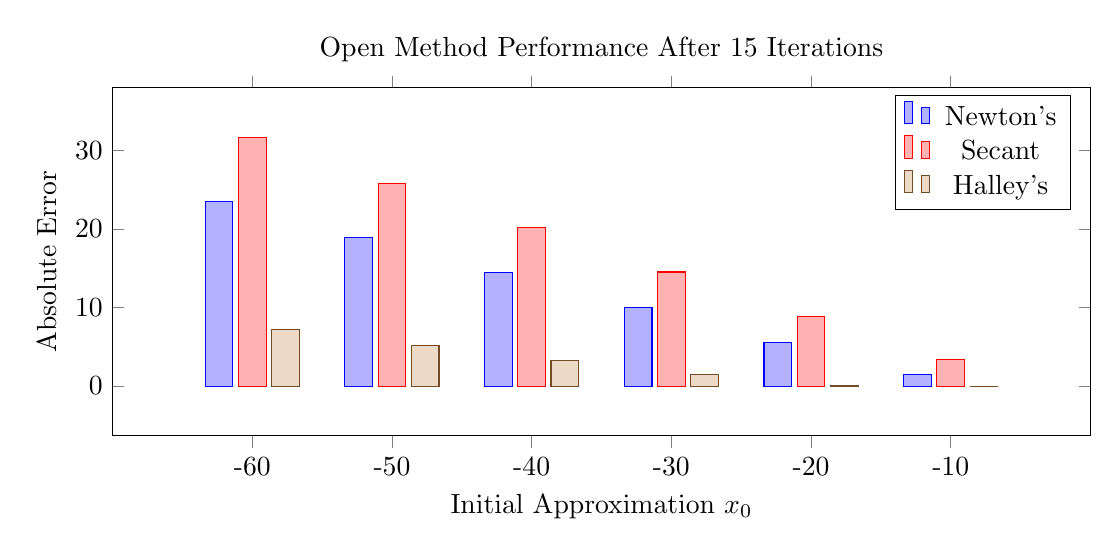
\begin{tikzpicture}
\begin{axis}[ybar, 
enlargelimits=0.2,
width=14cm,
height=6cm,
title={Open Method Performance After 15 Iterations},
xlabel={Initial Approximation $x_0$},
ylabel={Absolute Error},
symbolic x coords={-60,-50,-40,-30,-20,-10},
xtick=data,
]
\addplot coordinates {(-60,23.5) (-50,18.9) (-40,14.4) (-30,9.96) (-20,5.57)  (-10,1.521)};
\addplot coordinates {(-60,31.6) (-50,25.8) (-40,20.2) (-30,14.5) (-20,8.82)  (-10,3.384)};
\addplot coordinates {(-60,7.23) (-50,5.19) (-40,3.23) (-30,1.43) (-20,0.117) (-10,0)};
\legend{\ Newton's,\ Secant,\ Halley's}
\end{axis}
\end{tikzpicture}
\caption{Absolute error of various root-finders based on $x_0$ for the Wilkinson polynomial and known root $x=1$.}
\label{errorplot}
\end{figure}

It may be tempting to conclude there is a linear relationship between the absolute error and the initial approximation based, visually, on the graph. In reality, the relationship does appear \textit{approximately} linear for Newton's method and secant method \textit{on this particular interval}. Halley's method, however, is not approximately linear because the differences in error start quite large and then decrease rapidly as the initial approximation gets closer and closer to the true root.

Considering the absolute errors at initial guesses of $-60$ and $-10$, we can use the rate of change formula and slope-intercept formula to approximate the relationship between the absolute error (subscript $N$ for Newton's and $S$ for secant) and initial approximation in this specific case. The approximations are
\begin{align*}
    E_N(x_0) &\approx -0.44x_0 -2.87 \\
    E_S(x_0) &\approx -0.56x_0 -2.26
\end{align*}
for the interval $-60 \le x_0 \le -10$ we have considered. These results show that the simple Newton's method is fairly useful and comparable to methods such as secant method in this context. Also, Halley's method is well-equipped to deal with staring guesses that are far away from the root, in this specific case. Remember, however, that open-methods are not always guaranteed to converge like bracketed methods are. As mentioned previously, specifics such as the inputs to the algorithms and the polynomial or function itself are all factors that affect which method will converge the fastest; none of these methods are superior in all contexts and they all have advantages and disadvantages.  

\section{Conclusion}
\noindent
By understanding how two famous root-finders work, we able to explain why the bisection method must converge to a root in an interval and why horizontal regions pose a threat to Newton's method. Our Python code allowed for visualization of the two main methods, and we used important concepts such as the Fundamental Theorem of Algebra to solve root-finding problems. Additionally, we extended out study to a total of six algorithms and observed promising results for methods like TOMS748 and Halley's method. Using Wilkinson's polynomial and a limited number of iterations, we tracked absolute error remarked about its relationship to the initial approximation for open methods. Throughout, we observed that there is no usual ``best'' method, as each has the potential to outperform the others depending on the specifics of the problem and polynomial considered.

... % (NEXT STEPS)

\addcontentsline{toc}{section}{Acknowledgements}
\section*{Acknowledgements}
\noindent
Text.

\addcontentsline{toc}{section}{References}
% \begin{thebibliography}{40}

\bibitem{item1} Text.

\bibitem{item2} Text.

\end{thebibliography}

\newpage
\bibliographystyle{plain}
\bibliography{mybib}

\newpage
\appendix

\section{Appendix A}\label{manualalgorithms}
\noindent
Text.

\section{Appendix B}
\noindent
Text.

\end{document}